\documentclass[conference]{IEEEtran}
\usepackage[utf8]{inputenc}
\usepackage[T1]{fontenc}
\usepackage{amsmath, amsfonts, amssymb}
\usepackage[version=4]{mhchem}
\usepackage{graphicx}
\usepackage[export]{adjustbox}
\graphicspath{ {./images/} }

\title{Machine Learning-Based Assessment of NLFSR Cryptographic Strength Using NLFSR-Fingerprint Classification}

\author{
  \IEEEauthorblockN{Sultan Almuhammadi, Abdulmumin Sa'ad and Mohammed Mansour}
  \IEEEauthorblockA{
    Department of Computer Engineering,\\
    King Fahd University of Petroleum and Minerals,\\
    Dhahran, Saudi Arabia\\
    Email: \{muhamadi, g202203620, g202423860\}@kfupm.edu.sa
  }
}

\begin{document}

\maketitle

\begin{abstract}
Nonlinear Feedback Shift Registers (NLFSRs) are essential for stream-cipher security but, unlike LFSRs, offer no systematic way to infer their unknown Boolean feedback taps from outputs alone. We address this by simulating every $2^{n}-1$-length keystream of $n$-bit maximal-period NLFSRs across all nonzero seeds, converting each into a fixed-height binary image (with cyclic rotations), and training a compact CNN to map these stripe-patterns back to their tap configurations. This unified, end-to-end pipeline not only provides a practical NLFSR-fingerprinting tool but also reveals the deep structural geometry of maximum-period cycles and paves the way for ML-driven advances in NLFSR design and cryptanalysis.
\end{abstract}

\begin{IEEEkeywords}
NLFSR, cryptography, machine learning, convolutional neural networks, stream ciphers.
\end{IEEEkeywords}

\section{Introduction}
Nonlinear Feedback Shift Registers (NLFSRs) are fundamental building blocks in cryptographic stream ciphers, praised for their ability to generate long pseudorandom sequences from a compact hardware or software footprint. Unlike Linear Feedback Shift Registers (LFSRs), NLFSRs achieve higher algebraic complexity and resist classical linear cryptanalysis. However, designing NLFSRs with guaranteed maximum period $2^{n}-1$ remains an open challenge. This paper addresses the complementary problem of identifying feedback polynomials from keystream outputs using machine learning.

Machine learning, particularly deep learning, has shown remarkable success in pattern recognition tasks, making it a natural fit for analyzing the complex structures inherent in NLFSR-generated sequences. By converting keystreams into visual representations, such as binary images, convolutional neural networks (CNNs) can be trained to recognize unique patterns corresponding to specific feedback polynomials. This approach not only automates the classification process but also provides insights into the structural properties of NLFSRs, paving the way for advancements in cryptographic analysis and design.

\section{Related Work}

NLFSRs generalize the well-understood theory of LFSRs, whose maximum-period sequences arise from primitive polynomials. Dubrova (2012) catalogued quadratic NLFSRs, while Al-Hejri and Almuhammadi extended this to cubic feedback functions. On the cryptanalysis front, Kant et al. (2009) demonstrated machine learning-based attacks on LFSRs and certain classical generators like the Geffe and alternating step generators, showing high accuracy when predicting next bits using classifiers such as decision trees and neural networks. However, they also highlighted the limits of these methods against modern stream ciphers like Salsa20 and Rabbit, whose keystreams resisted ML-based prediction.

More recently, Jain et al. (2023) developed deep learning-based differential distinguishers for lightweight block ciphers like PRESENT and Simeck. Their approach used selected high-probability differentials to train neural networks to distinguish cipher outputs from random data, achieving high accuracy even with fewer rounds of encryption. Although their focus was on block ciphers, the framework of using structured differences and lightweight architectures informs our own ML pipeline design.

Our work integrates these elements into a unified ML-driven pipeline for NLFSR analysis, extending prior methods from block ciphers and LFSRs to analyze the relationship between NLFSR feedback configurations and their keystreams using classification models.

\section{Preliminaries}
An $n$-bit NLFSR consists of $n$ flip-flops and a nonlinear feedback function that determines the next state based on the current state. The feedback function can be represented as a Boolean polynomial, and the NLFSR's behavior depends on its initial state (seed) and feedback configuration. A maximal-period NLFSR generates a sequence of length $2^n - 1$ before repeating, provided the feedback function is carefully designed.

In this work, we focus on Fibonacci NLFSRs, where the feedback is applied to the first flip-flop, and the remaining flip-flops shift their contents sequentially. The keystream generated by an NLFSR is the sequence of bits output by the last flip-flop. By analyzing these keystreams, we aim to infer the feedback configuration using machine learning techniques.

\begin{figure}[ht]
  \centering
  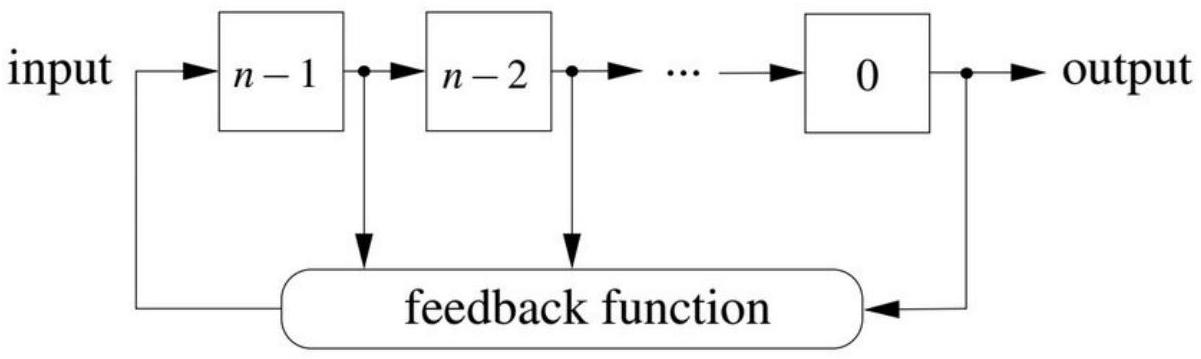
\includegraphics[max width=\columnwidth]{block_diagram.jpg}
  \caption{An $n$-bit FSR general structure.}
  \label{fig:block_diagram}
\end{figure}

\section{Methodology}
Our methodology involves the following steps:
\begin{enumerate}
  \item \textbf{Dataset Generation:} Simulate maximal-period NLFSRs for various feedback configurations and extract full-cycle keystreams for all nonzero seeds.
  \item \textbf{Image Encoding:} Convert each keystream into a fixed-height binary image, capturing cyclic rotations to preserve structural patterns.
  \item \textbf{Model Training:} Train a convolutional neural network (CNN) to classify feedback polynomials based on the encoded keystream images.
  \item \textbf{Evaluation:} Assess classification accuracy, analyze predictive features, and compare performance across different NLFSR sizes and configurations.
\end{enumerate}


\section{Results}
Preliminary results confirm the feasibility of our approach. Figure~\ref{fig:keystreams} shows 31 non-zero keystream plots produced by a 5-bit Fibonacci NLFSR with taps $[0,2,4,(2,3)]$. Each keystream exhibits unique local patterns, which our CNN leverages for classification.

\begin{figure}[ht]
  \centering
  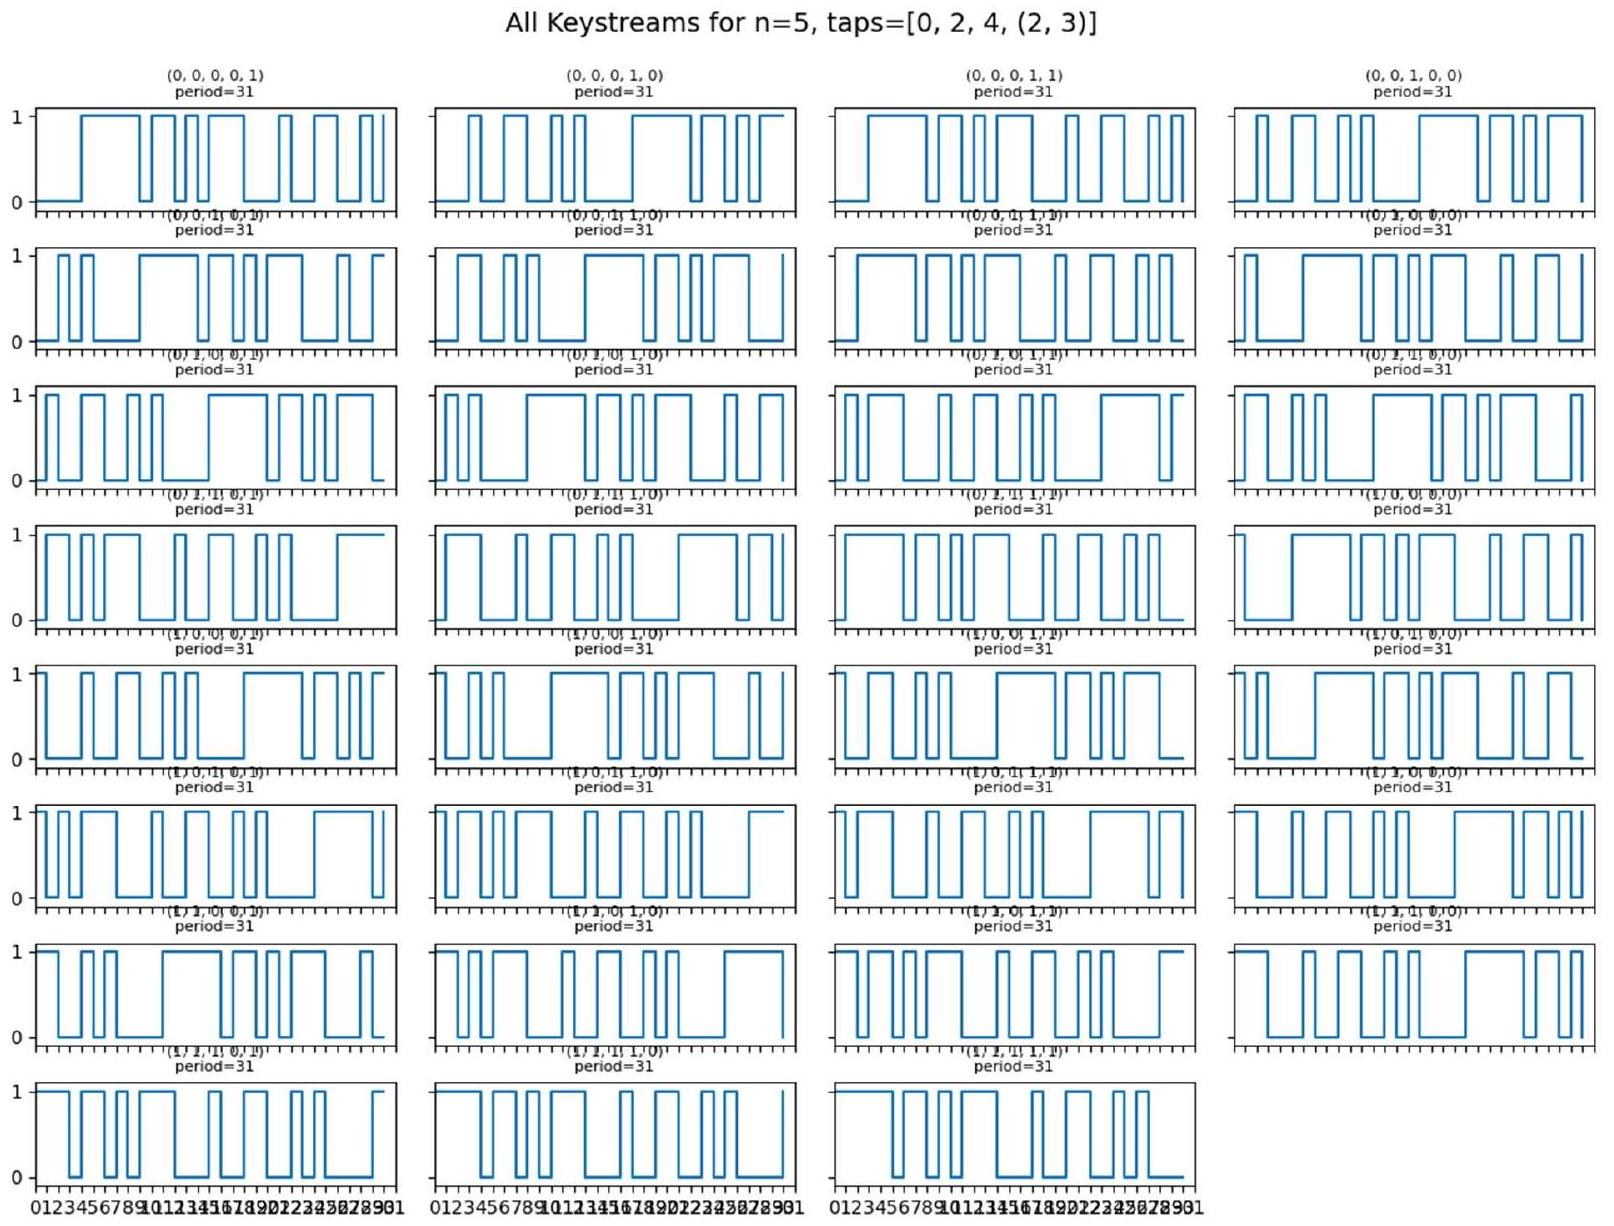
\includegraphics[max width=\columnwidth]{keystreams.jpg}
  \caption{31 Non-zero keystream plots for a 5-bit Fibonacci NLFSR.}
  \label{fig:keystreams}
\end{figure}

\section{Discussion}
Our approach demonstrates that each maximal-period feedback polynomial produces a unique "fingerprint" in its keystream. This insight advances NLFSR theory and provides a practical tool for cryptographic analysis. Challenges include scaling to larger $n$ and addressing class imbalance in the dataset.

\section{Conclusion}
This paper presents a novel ML-based pipeline for NLFSR analysis, combining exhaustive dataset generation, image encoding, and CNN classification. Future work will focus on scaling the methodology and exploring its applicability to other cryptographic primitives.

\section*{Acknowledgment}
The authors thank King Fahd University of Petroleum and Minerals for supporting this research.

\bibliographystyle{IEEEtran}
\bibliography{references}

\end{document}
